%!TEX root = ../../main.tex

\chapter{Anleitung für Verwaltungsangestellte}
\label{sec:chap1}
\section{Kursübersicht}
Der Benutzer kann zu jedem Zeitpunkt zur Kursübersicht gelangen. Diese ist in der Menüleiste im Sandwichmenü zu den Kursen zu finden.\\
In der Kursübersicht findet der Benutzer alle Kurse. Diese sind je nach Anzahl auf verschiedene Seiten aufgeteilt. Ein Wechsel zwischen den Seiten kann durch Klicken auf die jeweilige Seitenzahl erfolgen. Ein Beispiel einer Kursübersicht für einen Administrator findet sich in Abbildung \ref{fib:kü}.

\begin{figure}[h]
\centering
\includegraphics[height=.5\textwidth]{kursübersicht_verwaltungsangestellter.png}
\caption{Kursübersicht für Verwaltungsangestellte}
\label{fib:kü}
\end{figure}

Um genauere Informationen zum jeweiligen Kurs zu erhalten, muss der Benutzer den Kurs durch klicken auf die Ausklappschaltfläche ausklappen (siehe Abbildung \ref{fib:kü-ausgeklappt}). Dadurch werden dem Verwaltungsangestellten alle Mitglieder des Kurses sowie die gestellten Aufgaben angezeigt. Hier können durch klicken der Schaltfläche \glqq Anzeigen\grqq{} weitere Informationen zur Aufgabe angezeigt werden. 

\begin{figure}[h]
\centering
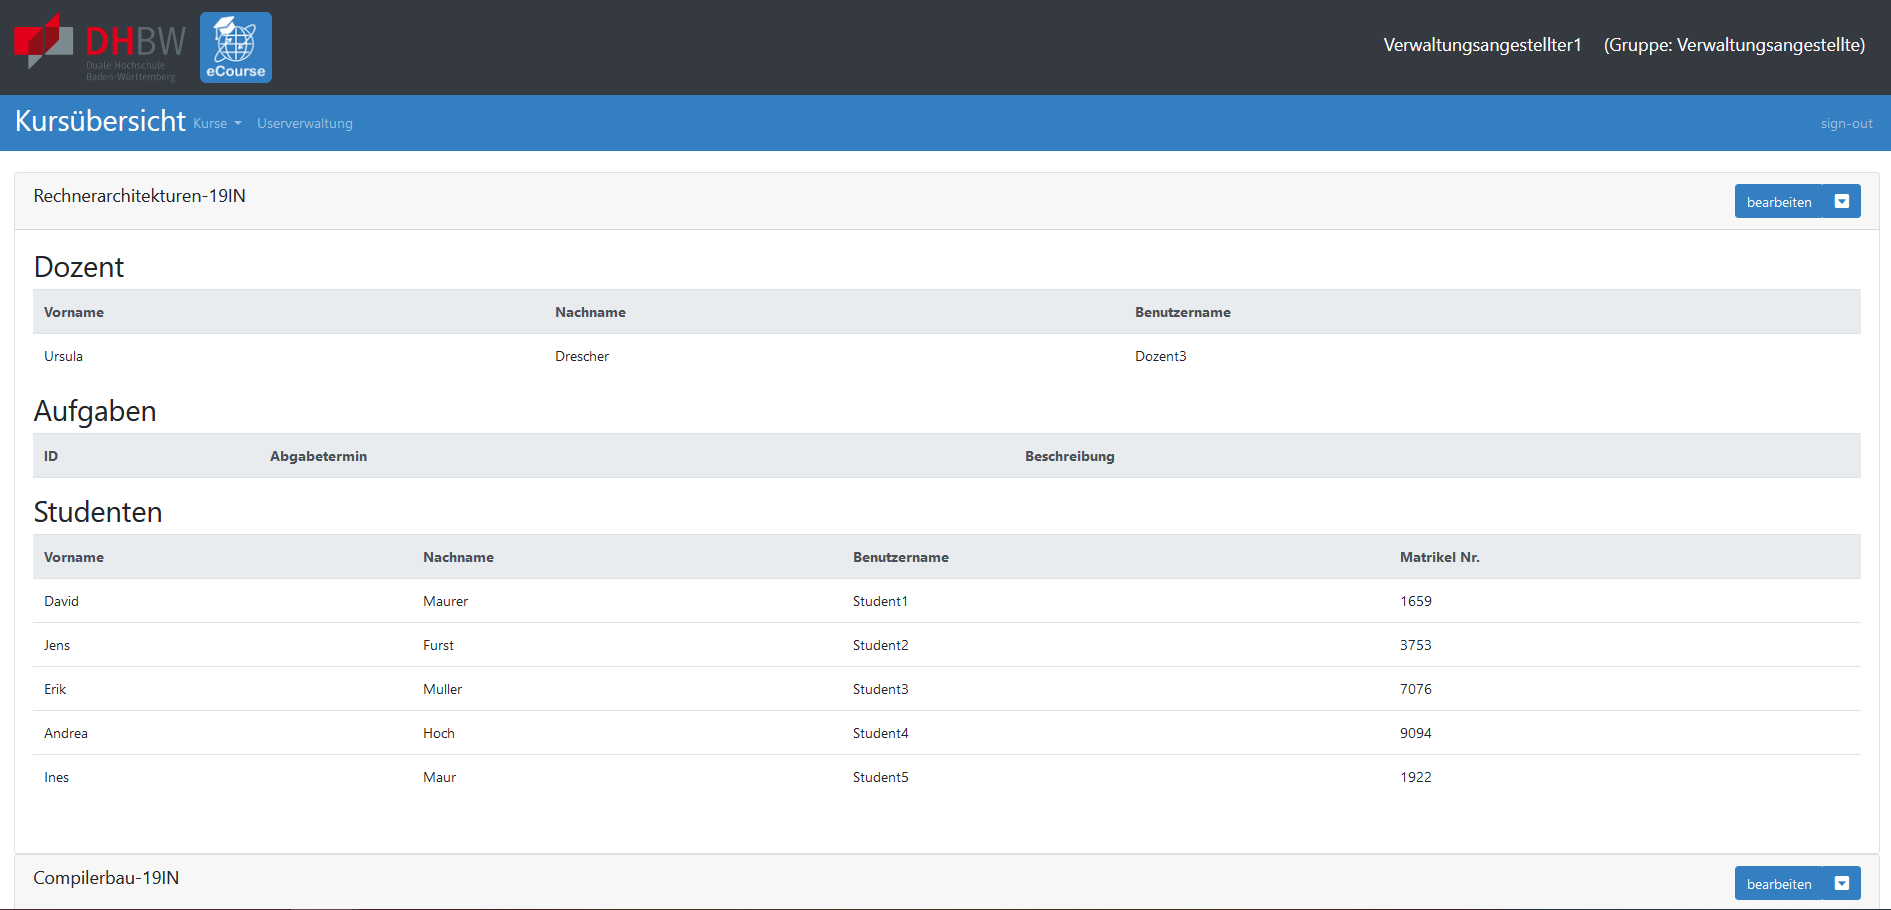
\includegraphics[height=.5\textwidth]{kurs_ausgeklappt_verwaltungsangestellter.png}
\caption{Ausgeklappte Kursübersicht für Verwaltungsangestellte}
\label{fib:kü-ausgeklappt}
\end{figure}

\section{Kurs anlegen}
Ebenfalls im Untermenü Kurse ist die Möglichkeit zum Kurse anlegen gegeben.\\
Ein Kurs kann angelegt werden, wenn das angezeigte Formular (siehe Abbildung \ref{fib:ke}) ausgefüllt wird. Es muss ein Dozent ausgewählt werden. Dieser kann im Dropdown-Menü aus einer Liste aller Dozenten ausgewählt werden. \\
Die Teilnehmer am Kurs aus der Gruppe der Studierenden werden hinzugefügt, indem man sie anhand ihres Benutzernamens in der Liste ausfindig macht und mit einem Haken versieht. \\
Außerdem sollte dem Kurs sinnvoller Name vergeben werden. Von den Entwicklern wird ein Name empfohlen der dem folgenden Schema entspricht: \\
\verb/Kursname_JJKursbezeichnung/
Abschließend kann über einen Kalender ein Start- und Enddatum des Kurses festgelegt werden. 
Die Erstellung des Kurses kann durch klicken der Schaltfläche \glqq Kurs erstellen\grqq{} beendet werden.

\begin{figure}[h]
\centering
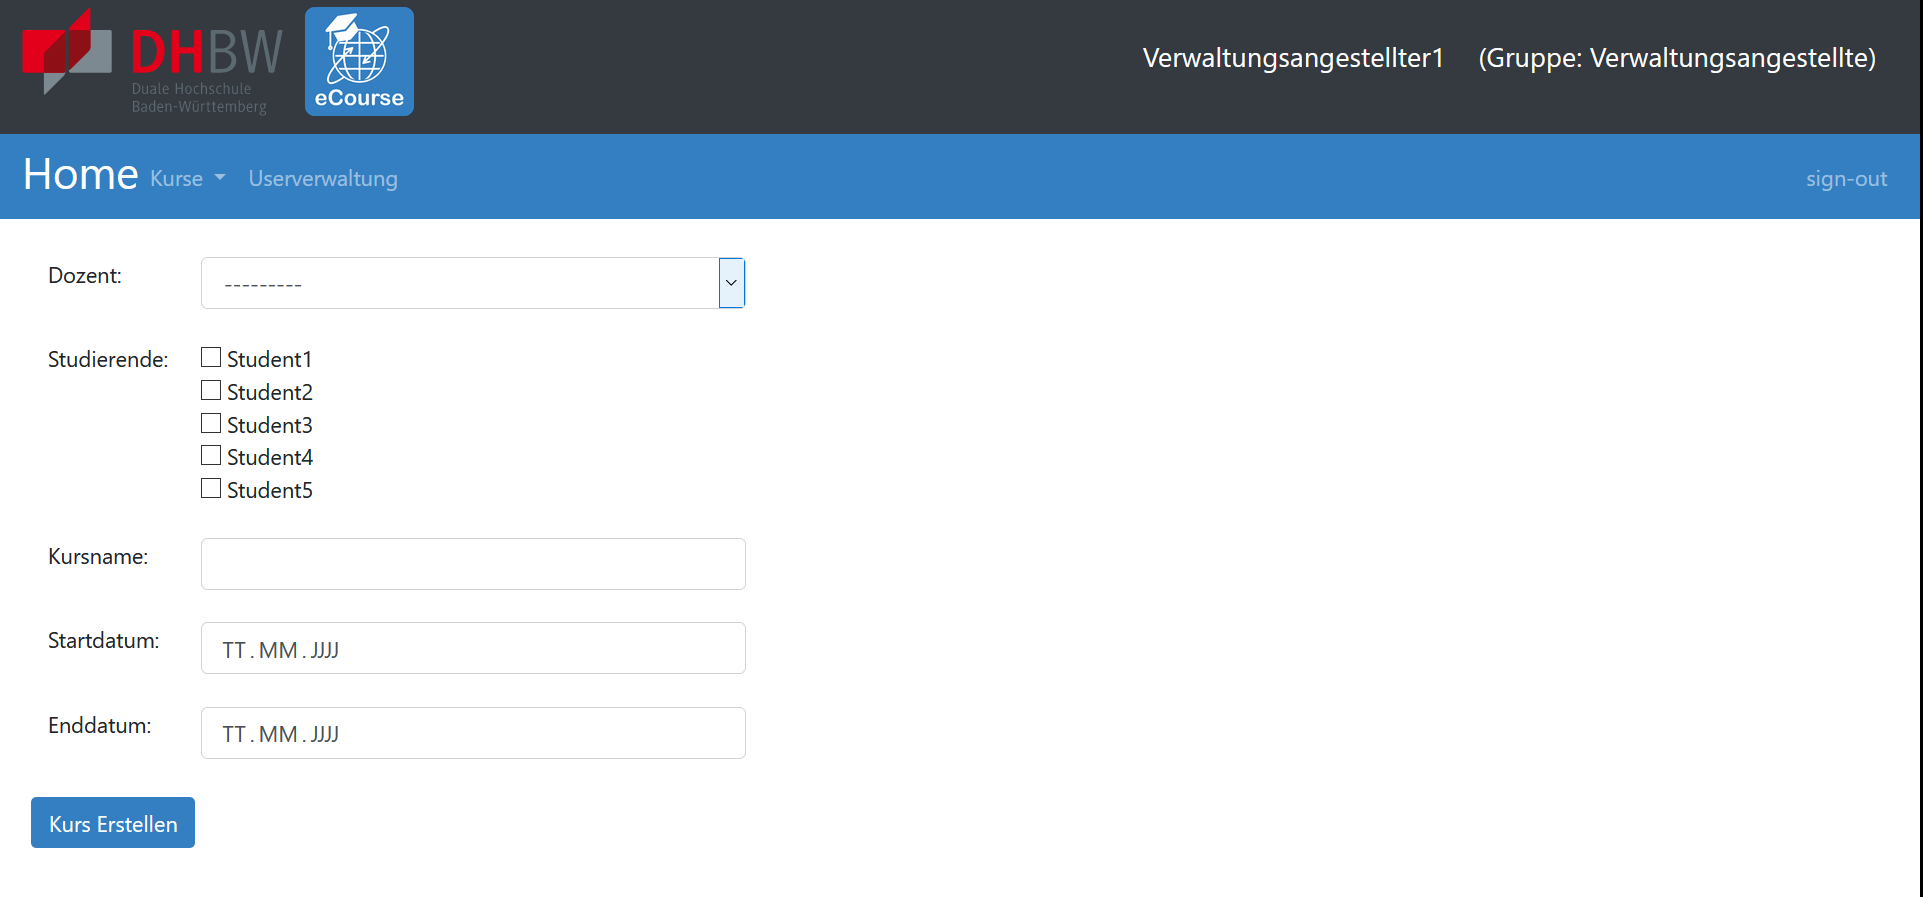
\includegraphics[height=.5\textwidth]{kurs_anlegen_verwaltungsangestellter.png}
\caption{Kurs anlegen durch Verwaltungsangestellten in der Anwendung eCourse}
\label{fib:ke}
\end{figure}


\section{Kurs bearbeiten}
Kurse können nur bearbeitet werden, wenn sich der Benutzer in der Kursübersicht befindet. Dort findet sich neben jedem Kursnamen eine Schaltfläche \glqq bearbeiten\grqq . Wird diese betätigt öffnet sich das gleiche Formular wie auch bei der Kurserstellung. Im Gegensatz zum Anlegen des Kurses ist das Formular aber hier mit den Informationen über den Kurs gefüllt und kann bei Bedarf abgeändert werden.\\
Wurden Änderungen vorgenommen, werden diese gespeichert in dem der Nutzer die Schaltfläche \glqq Speichern\grqq{} betätigt.\\
Möchte der Benutzer keine Änderungen vornehmen, kann er über die Schaltfläche \glqq Zurück\grqq{} zurück auf die Kursübersicht gelangen.
Außerdem können hier auch Kurse gelöscht werden. Dies sollte unter größter Sorgfalt geschehen, da die Betätigung der Schaltfläche \glqq Löschen\grqq{} zum sofortigen Löschen des Kurses führt. Die Löschung eines Kurses wird durch das Anzeigen einer Erfolgsmeldung bestätigt (siehe Abbildung \ref{fib:kl}). Über betätigen der dort angezeigten \glqq zurück\grqq{} Schaltfläche gelangt der Nutzer wieder zurück auf die Kursübersicht.

\begin{figure}[h]
\centering
\includegraphics[height=.5\textwidth]{kurs_gelöscht.png}
\caption{Erfolgsmeldung Kurs gelöscht in der Anwendung eCourse}
\label{fib:kl}
\end{figure}

\section{Benutzerübersicht}
Die Benutzerübersicht kann ebenfalls zu jeder Zeit erreicht werden, indem der Benutzer in der Menüleiste den Punkt \glqq Userverwaltung\grqq{} anklickt. Ein Beispiel einer Benutzerverwaltung ist in Abbildung \ref{fib:userverwaltung} dargestellt.
Die Benutzerübersicht ist aufgeteilt in 4 Bereiche: die Studentenliste, die Dozentenliste, die Admin- und Mitarbeiterliste und den Punkt Benutzer erstellen. \\
In den jeweiligen Listen werden alle Benutzer aufgeführt, die den jeweils angegebenen Benutzertyp haben. Die Liste der Benutzer ist analog zu der Liste der Kurse auf mehrere Seiten aufgeteilt, wobei die jeweiligen Seiten über klicken auf die verschiedenen Seitennummern erreicht werden können.\\
Die Listen können durch verschiedene Filterfunktionen (siehe Abbildung \ref{fib:filter})nach bestimmten Nutzern durchsucht werden. 
\begin{figure}[h]
\centering
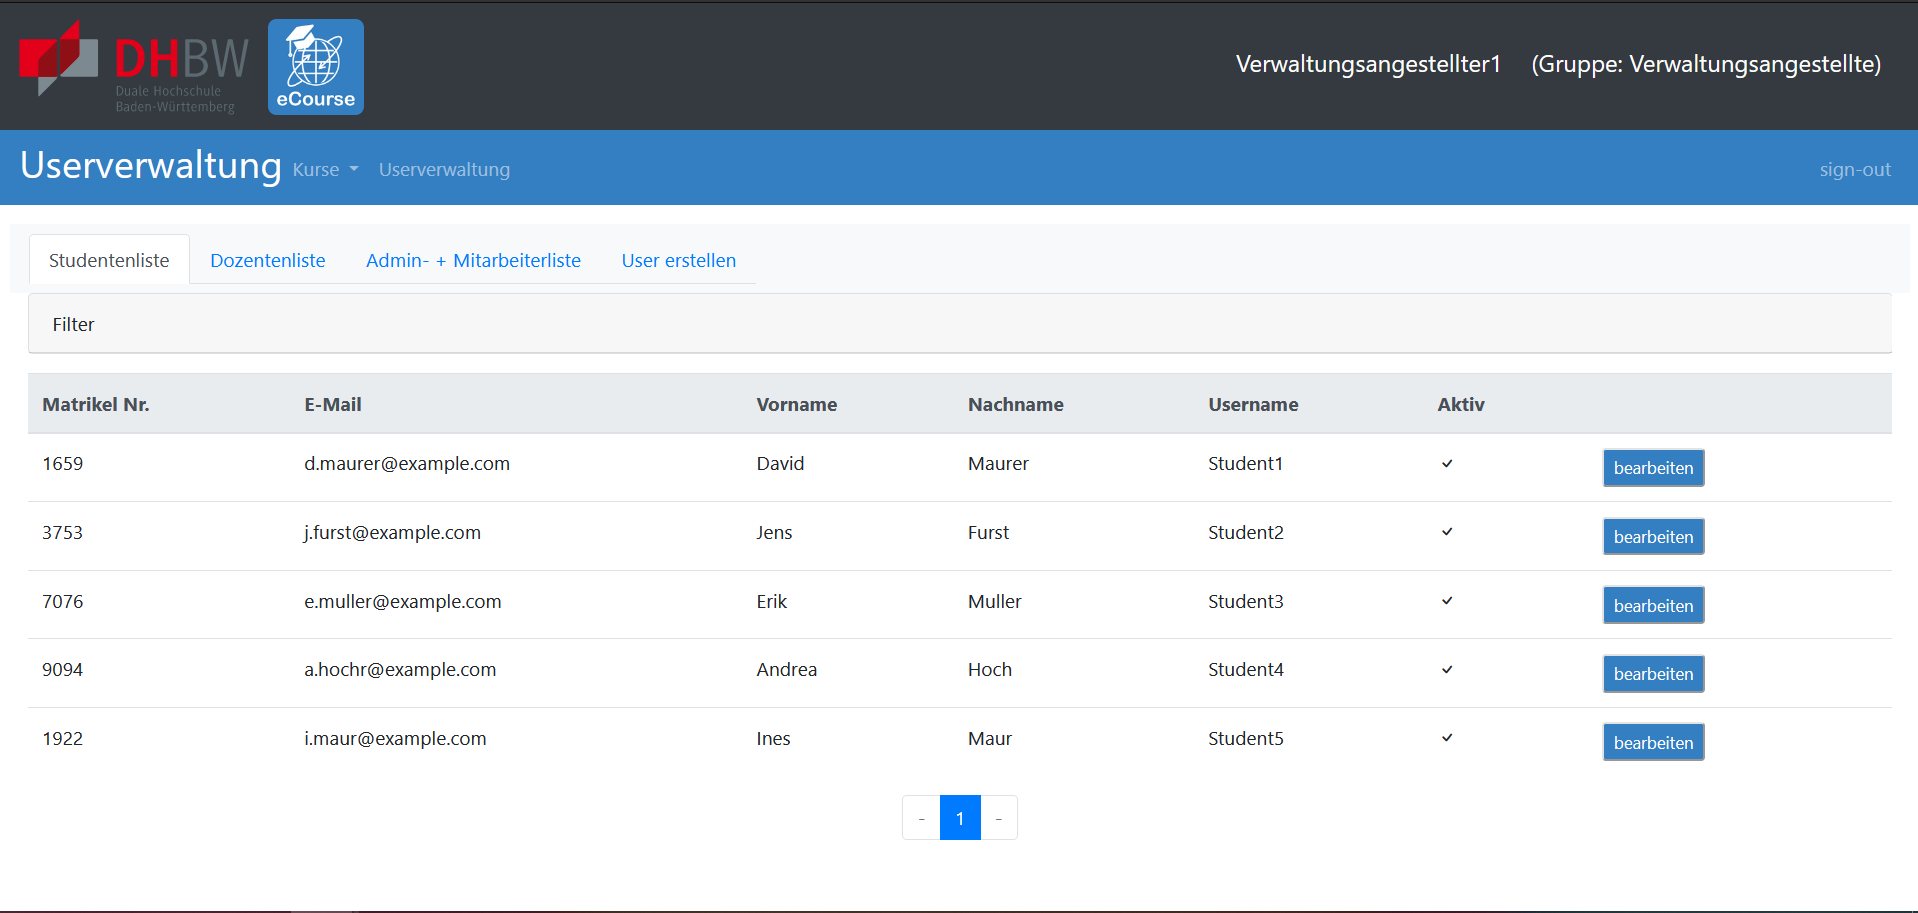
\includegraphics[height=.5\textwidth]{userverwaltung.png}
\caption{Benutzerverwaltung in der Anwendung eCourse}
\label{fib:userverwaltung}
\end{figure}

\begin{figure}[h]
\centering
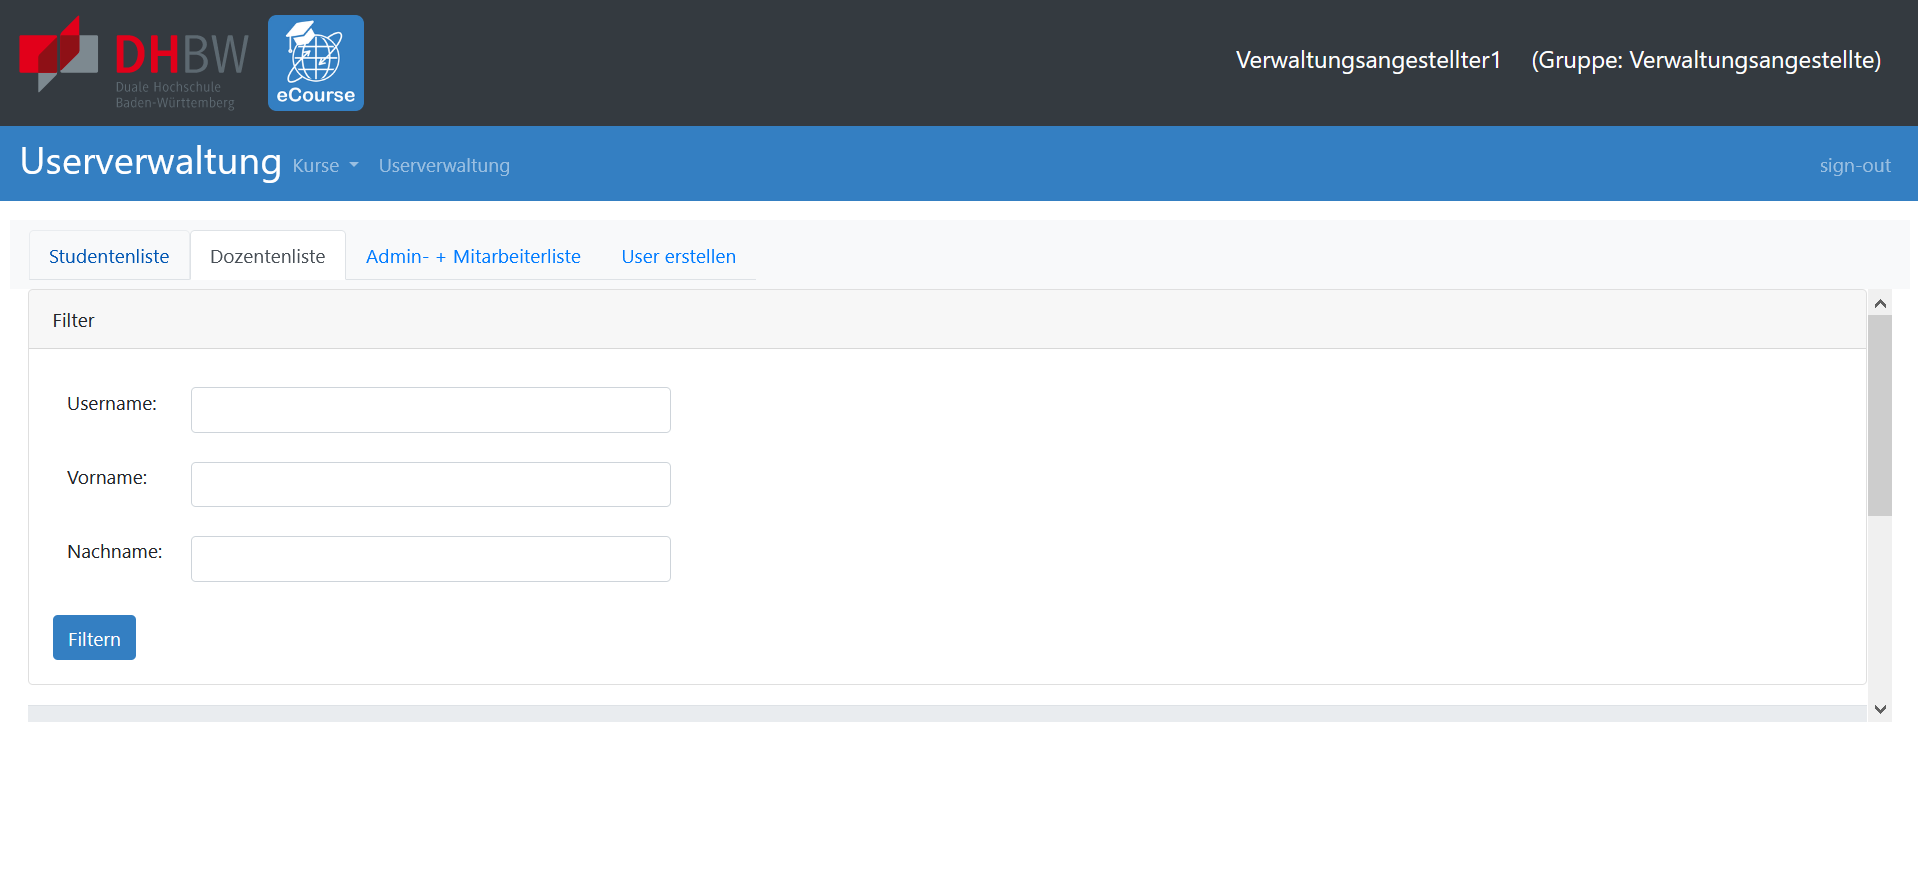
\includegraphics[height=.5\textwidth]{filter_userverwaltung.png}
\caption{Filterfunktion für die Benutzerverwaltung in der Anwendung eCourse}
\label{fib:filter}
\end{figure}


\section{Benutzer anlegen}
Im Unterpunkt \glqq User erstellen\grqq\: der Benutzerverwaltung können Benutzer erstellt werden. Bei der Erstellung wird unabhängig vom Benutzertyp ein Benutzername, ein Vorname, ein Nachname und eine E-Mail-Adresse verlangt. Nur der Gruppe der Studierenden erhält zusätzlich noch eine Matrikelnummer (siehe Abbildung \ref{fib:benutzer_erstellen}). Der Benutzertyp selbst wird aus einem Drop-Down-Menü ausgewählt. Es stehen Verwaltungsangestellter, Studierender und Dozierender zur Verfügung als möglicher Benutzertyp. \\
Wichtig zu beachten ist, wurde ein Benutzer erstellt, taucht er in der entsprechenden Liste erst dann auf, wenn die Seite manuell aktualisiert wurde. Diese Maßnahme wurde eingebaut um die Performanz der Seite zu verbessern.

\begin{figure}[h]
\centering
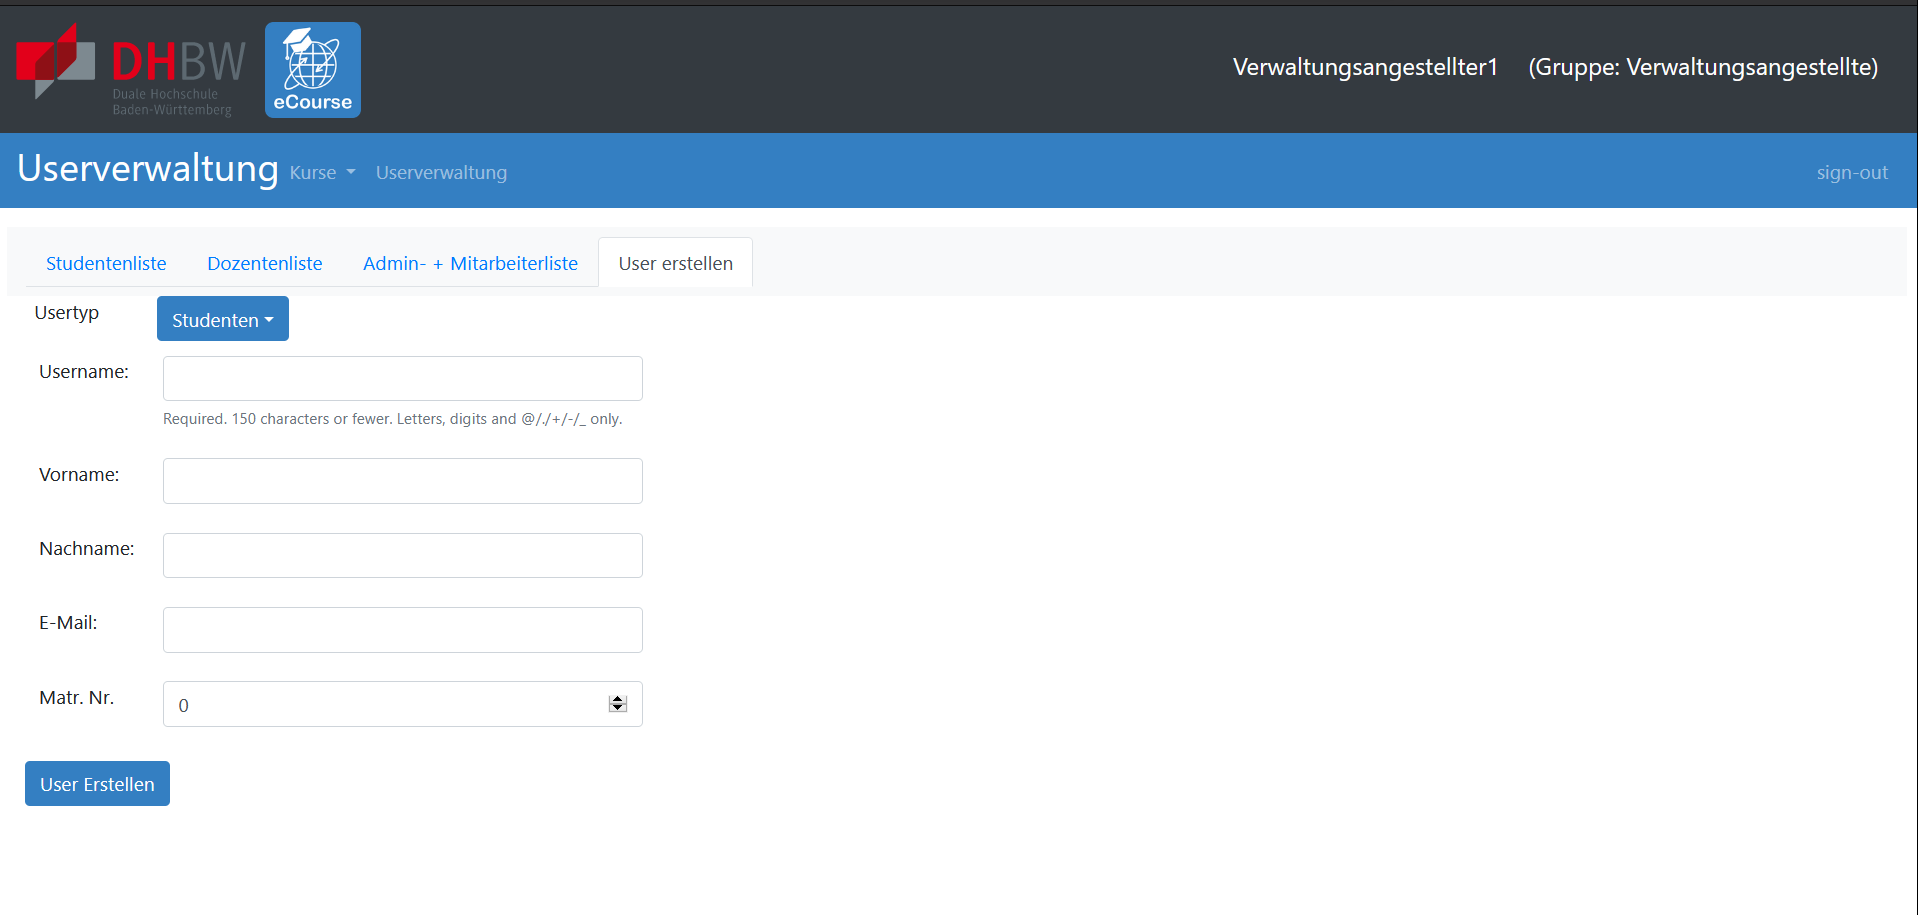
\includegraphics[height=.5\textwidth]{user_erstellen.png}
\caption{Benutzer erstellen am Beispiel eines Studenten}
\label{fib:benutzer_erstellen}
\end{figure}

\section{Benutzer bearbeiten}
In den jeweiligen Listen können die Benutzer nun auch bearbeitet werden. Dies kann nötig sein, wenn zum Beispiel ein Benutzer seine E-Mail-Adresse ändert. Die Maske zur Bearbeitung eines Benutzers ist in Abbildung \ref{fib:user_bearbeiten} dargestellt.\\
Die Bearbeitung eines Benutzers geschieht analog zur Bearbeitung der Kurse, allerdings wird die Bearbeitung der Nutzer nicht auf einer neuen Seite ausgeführt, sondern in einem Pop-up Fenster. Muss also ein Nutzer bearbeitet werden, muss er zuerst in der Liste gefunden werden. Dann kann über die Betätigung der Schaltfläche \glqq bearbeiten\grqq{} die Bearbeitung aktiviert werden. Hier können nun alle Informationen über den Benutzer verändert werden.\\ Die Bearbeitung kann abgeschlossen werden durch Betätigung der Schaltfläche \glqq Speichern\grqq . Möchte der Benutzer die Bearbeitung abbrechen, kann er dies zu jedem  Zeitpunkt tun, indem er das Pop-up Fenster mit einem Klick auf das \glqq x\grqq{} schließt.\\
Auch hier kann der Benutzer analog zu den Kursen den Benutzer löschen. Auch hier ist zu beachten, dass der Benutzer direkt nach Betätigung der Schaltfläche \glqq Löschen\grqq{} gelöscht wird. Die Schaltfläche sollte also nur betätigt werden, wenn der Benutzer auch wirklich gelöscht werden soll.\\
Ist der Benutzer erfolgreich gelöscht, wird dies durch eine Erfolgsmeldung wie in Abbildung \ref{fib:user_löschen} gezeigt bestätigt.
Nach der Bearbeitung eines Benutzers muss wie auch bei der Erstellung die Seite neu geladen werden, um die Veränderungen auch in der Liste sehen zu können.\\

\begin{figure}[h]
\centering
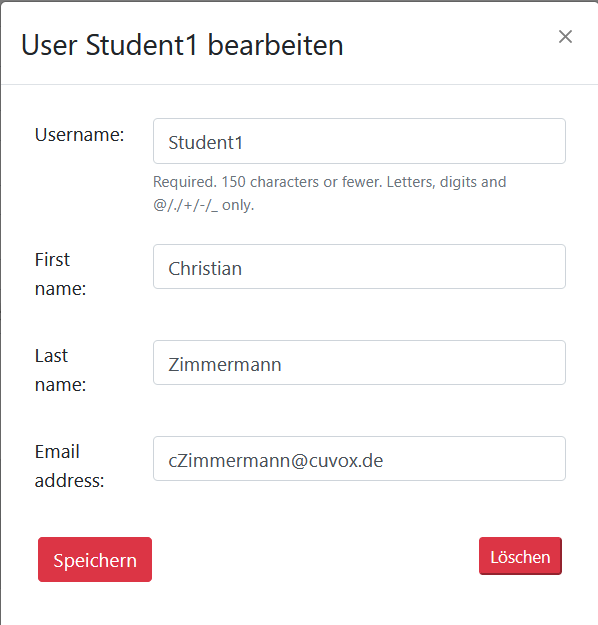
\includegraphics[height=.5\textwidth]{user_bearbeiten.png}
\caption{Bearbeiten eines Benutzers am Beispiel eines Studenten}
\label{fib:user_bearbeiten}
\end{figure}

\begin{figure}[h]
\centering
\includegraphics[height=.5\textwidth]{user_löschen_erfolgreich.png}
\caption{Erfolgsmeldung Benutzer gelöscht in der Anwendung eCourses}
\label{fib:user_löschen}
\end{figure}